\documentclass{article}
\usepackage[left=0.5in,top=0.5in,right=0.5in,bottom=0.5in]{geometry}
\usepackage[english]{babel}
\usepackage[utf8]{inputenc}
\usepackage[table]{xcolor}
\usepackage{amssymb,amsmath,amsthm}
\usepackage{changepage,threeparttable}
\usepackage{booktabs,multirow}
\usepackage{graphicx}
\usepackage{soul}
\graphicspath{{./images/}}
\def\R#1#2{\(R_{\text{\tiny#1,\tiny#2}}(\Omega)\)}
\def\RTH#1#2{R_{\text{\tiny#1,\tiny#2}} (\Omega)}
\def\RP#1{R_{\text{\tiny#1}}}
\def\RS#1{R_{\text{\tiny#1}}}
\def\OHMs{~\Omega}
\def\OHM{~\(\Omega \)}
\title{Lab 4: Resistor Networks}
\author{Philip Kim}
\date{\today}
\begin{document}
\maketitle
\vspace*{-1cm}
\begin{table}[!htp]\centering
  \subsection*{Part 1}
  \begin{tabular}{|c|c|c|c|c|c|c|}\hline
  \multicolumn{6}{|c|}{\textbf{Table 1: Parallel Networks}} \\\hline
  \R{1}{th} & \R{1}{exp} & \R{2}{th} & \R{2}{exp} & \R{P}{th} & \R{P}{exp} \\\hline
  1k & 0.99k & 2k & 1.99k & 0.67k & 0.67k \\\hline
  1k & 0.99k & 510 & 0.51k & 0.34k & 0.36k \\\hline
  1k & 0.99k & 3.3k & 3.29k & 0.77k & 0.77k \\\hline
  10k & 9.97k & 5.1k & 5.07k & 3.36k & 3.36k \\\hline
  10k & 9.97k & 20k & 19.94k & 6.65k & 6.62k \\\hline
  10k & 9.97k & 47k & 47.40k & 8.24k & 8.20k \\\hline
  \end{tabular}
  \begin{center}
    \subsection*{Picture 1: \R{1}{exp},~\R{2}{exp},~\R{P}{exp}}
    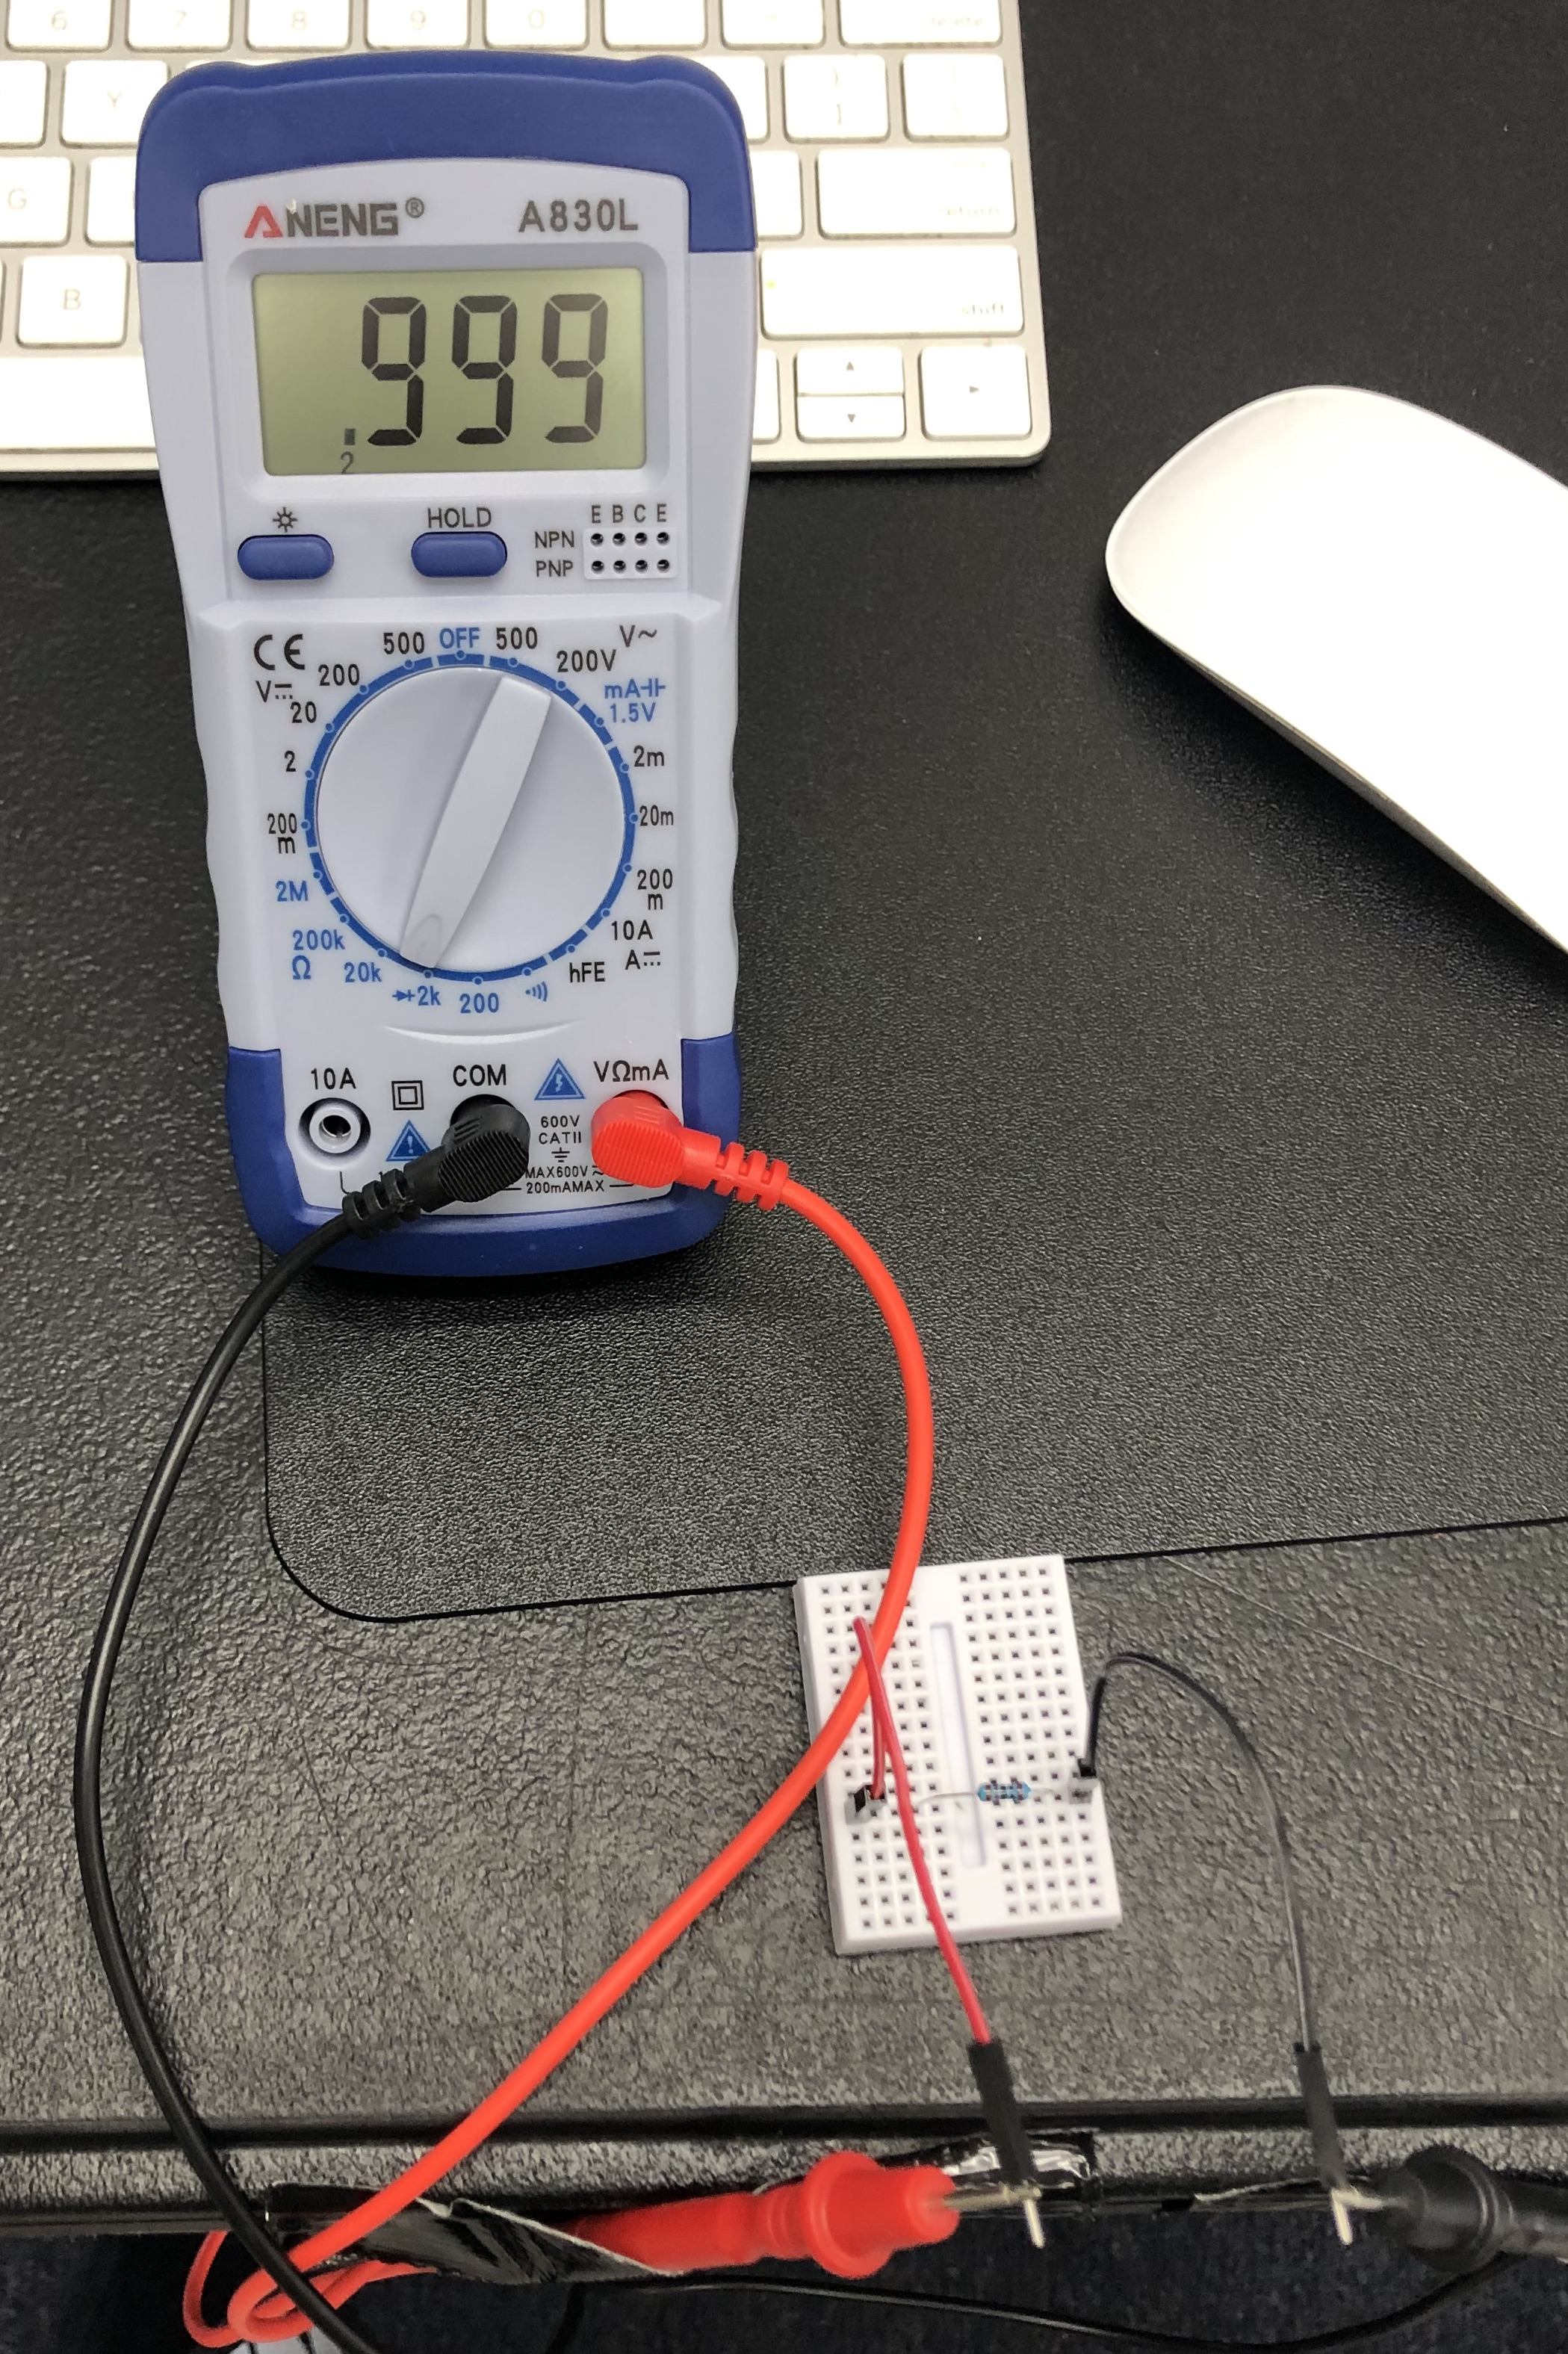
\includegraphics[scale=0.079,height=4.5cm]{R1.jpeg}
    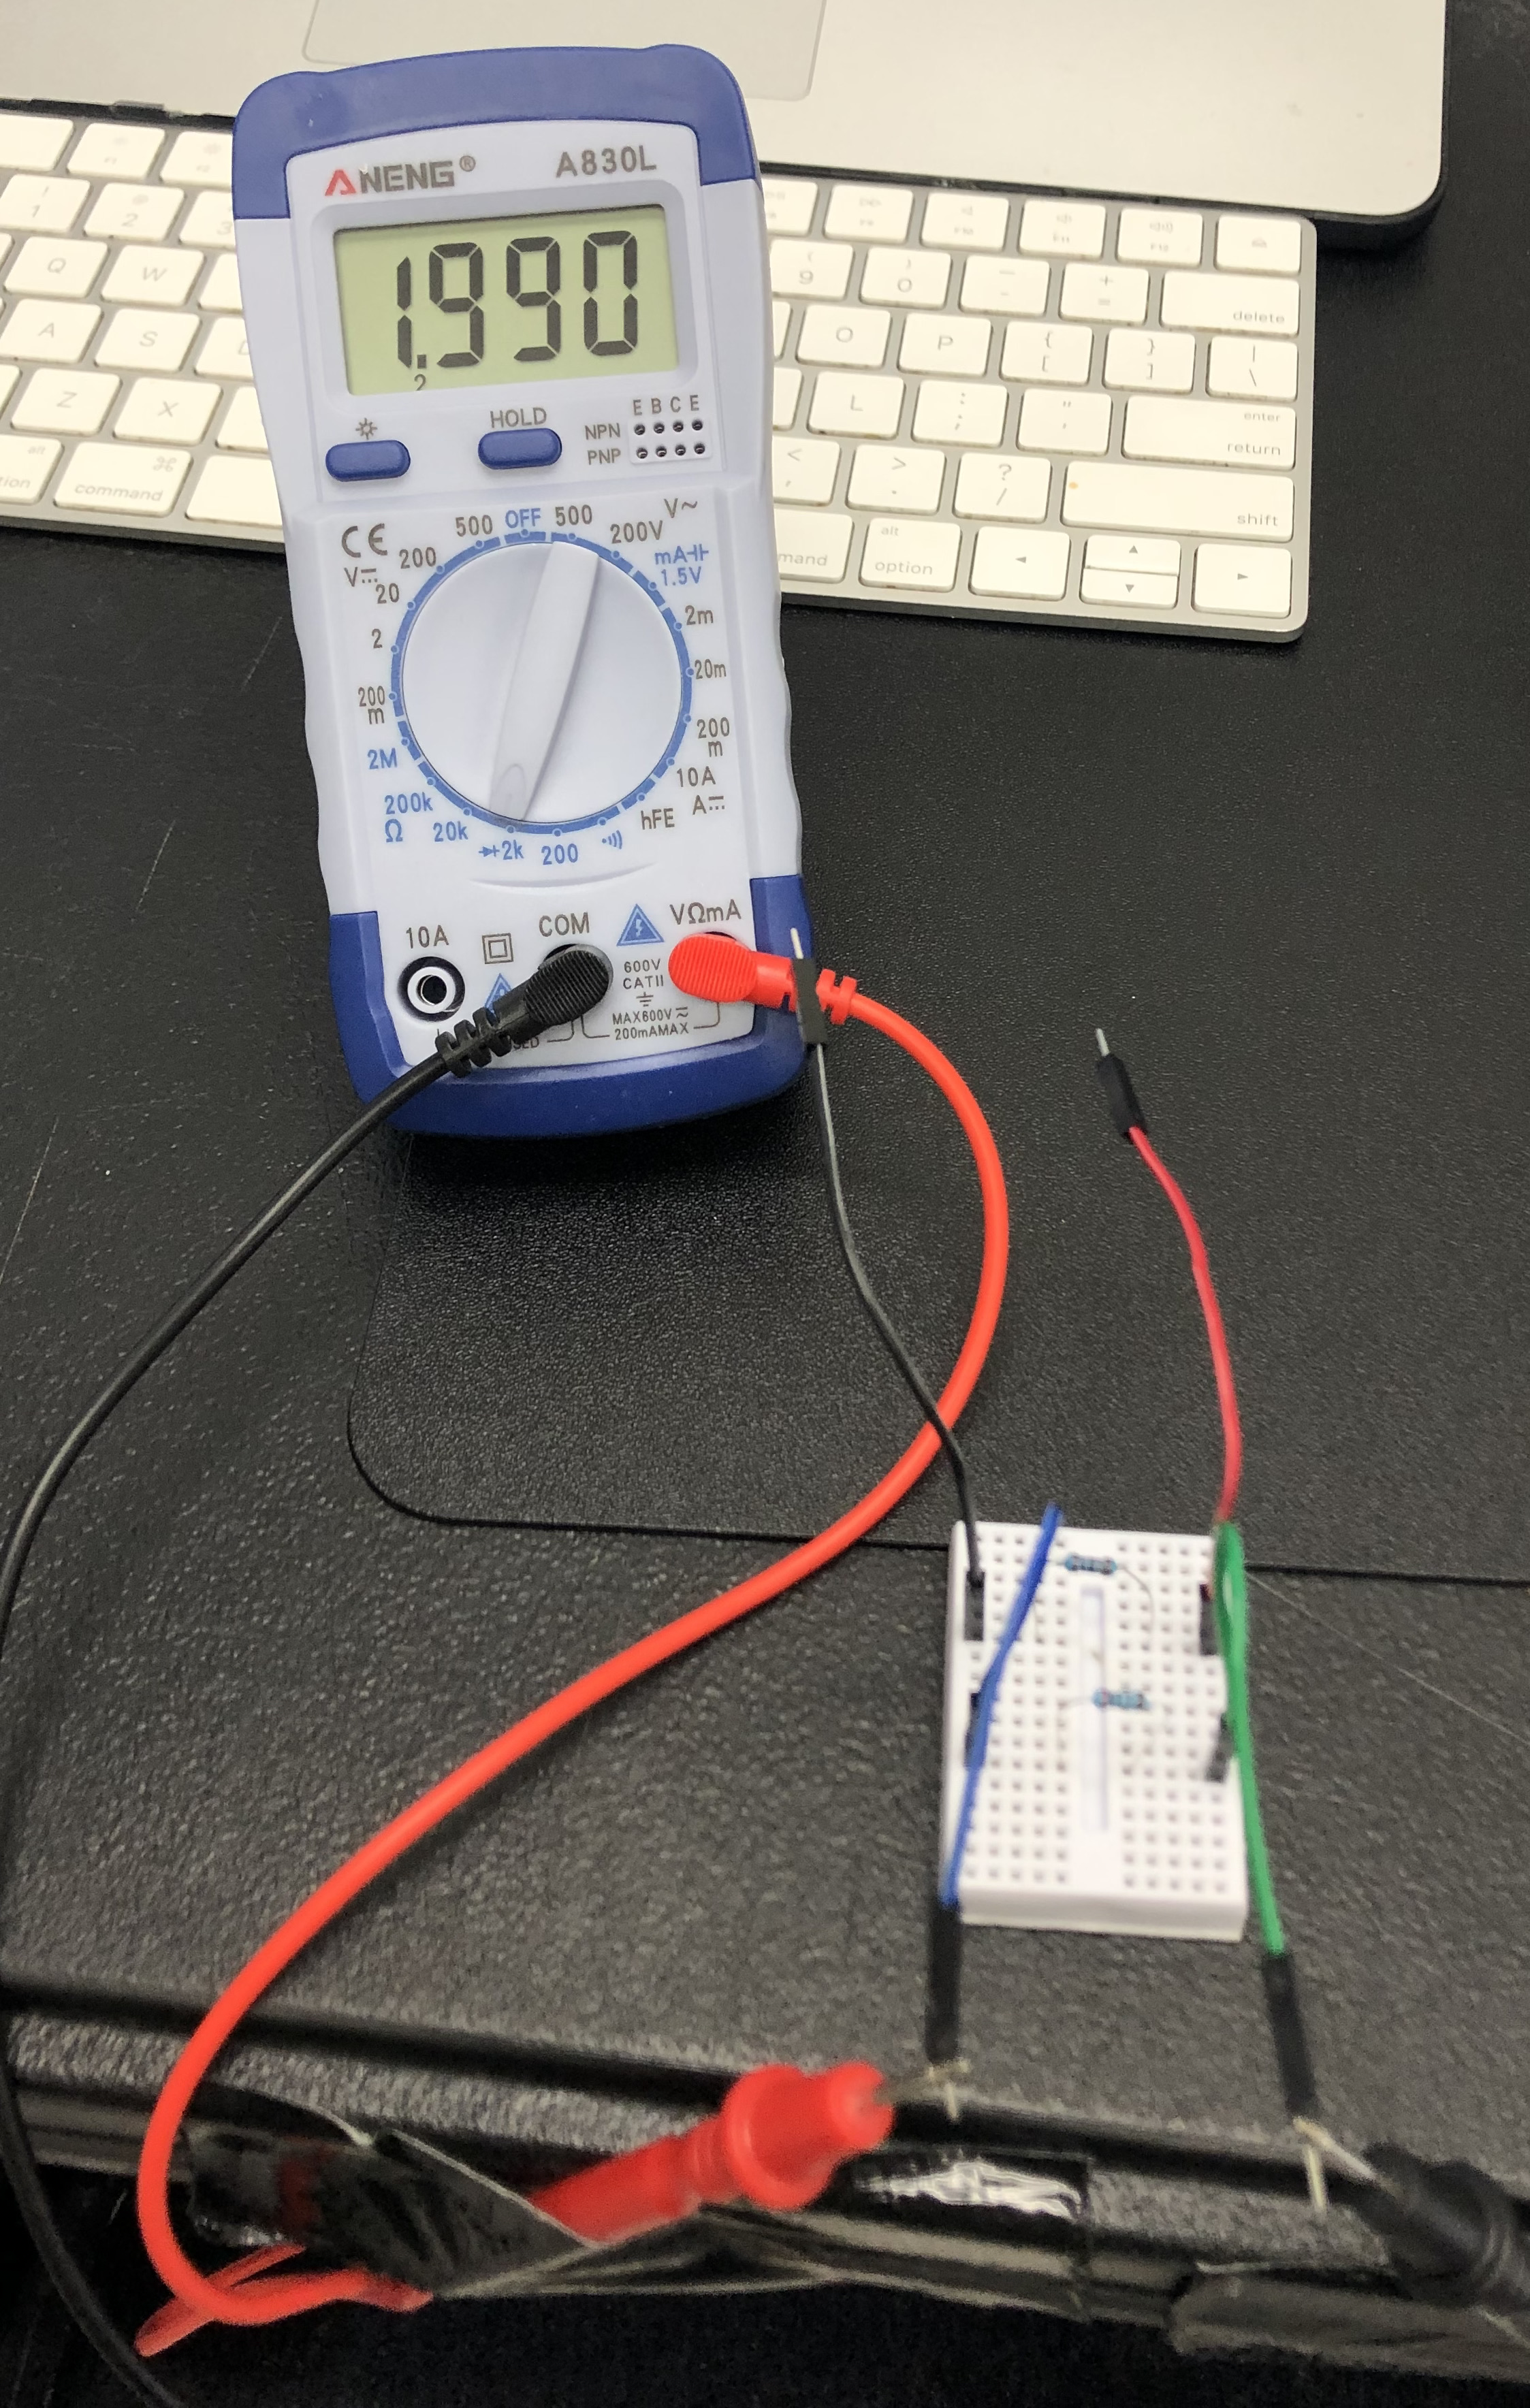
\includegraphics[scale=0.070,height=4.5cm]{R2.jpeg}
    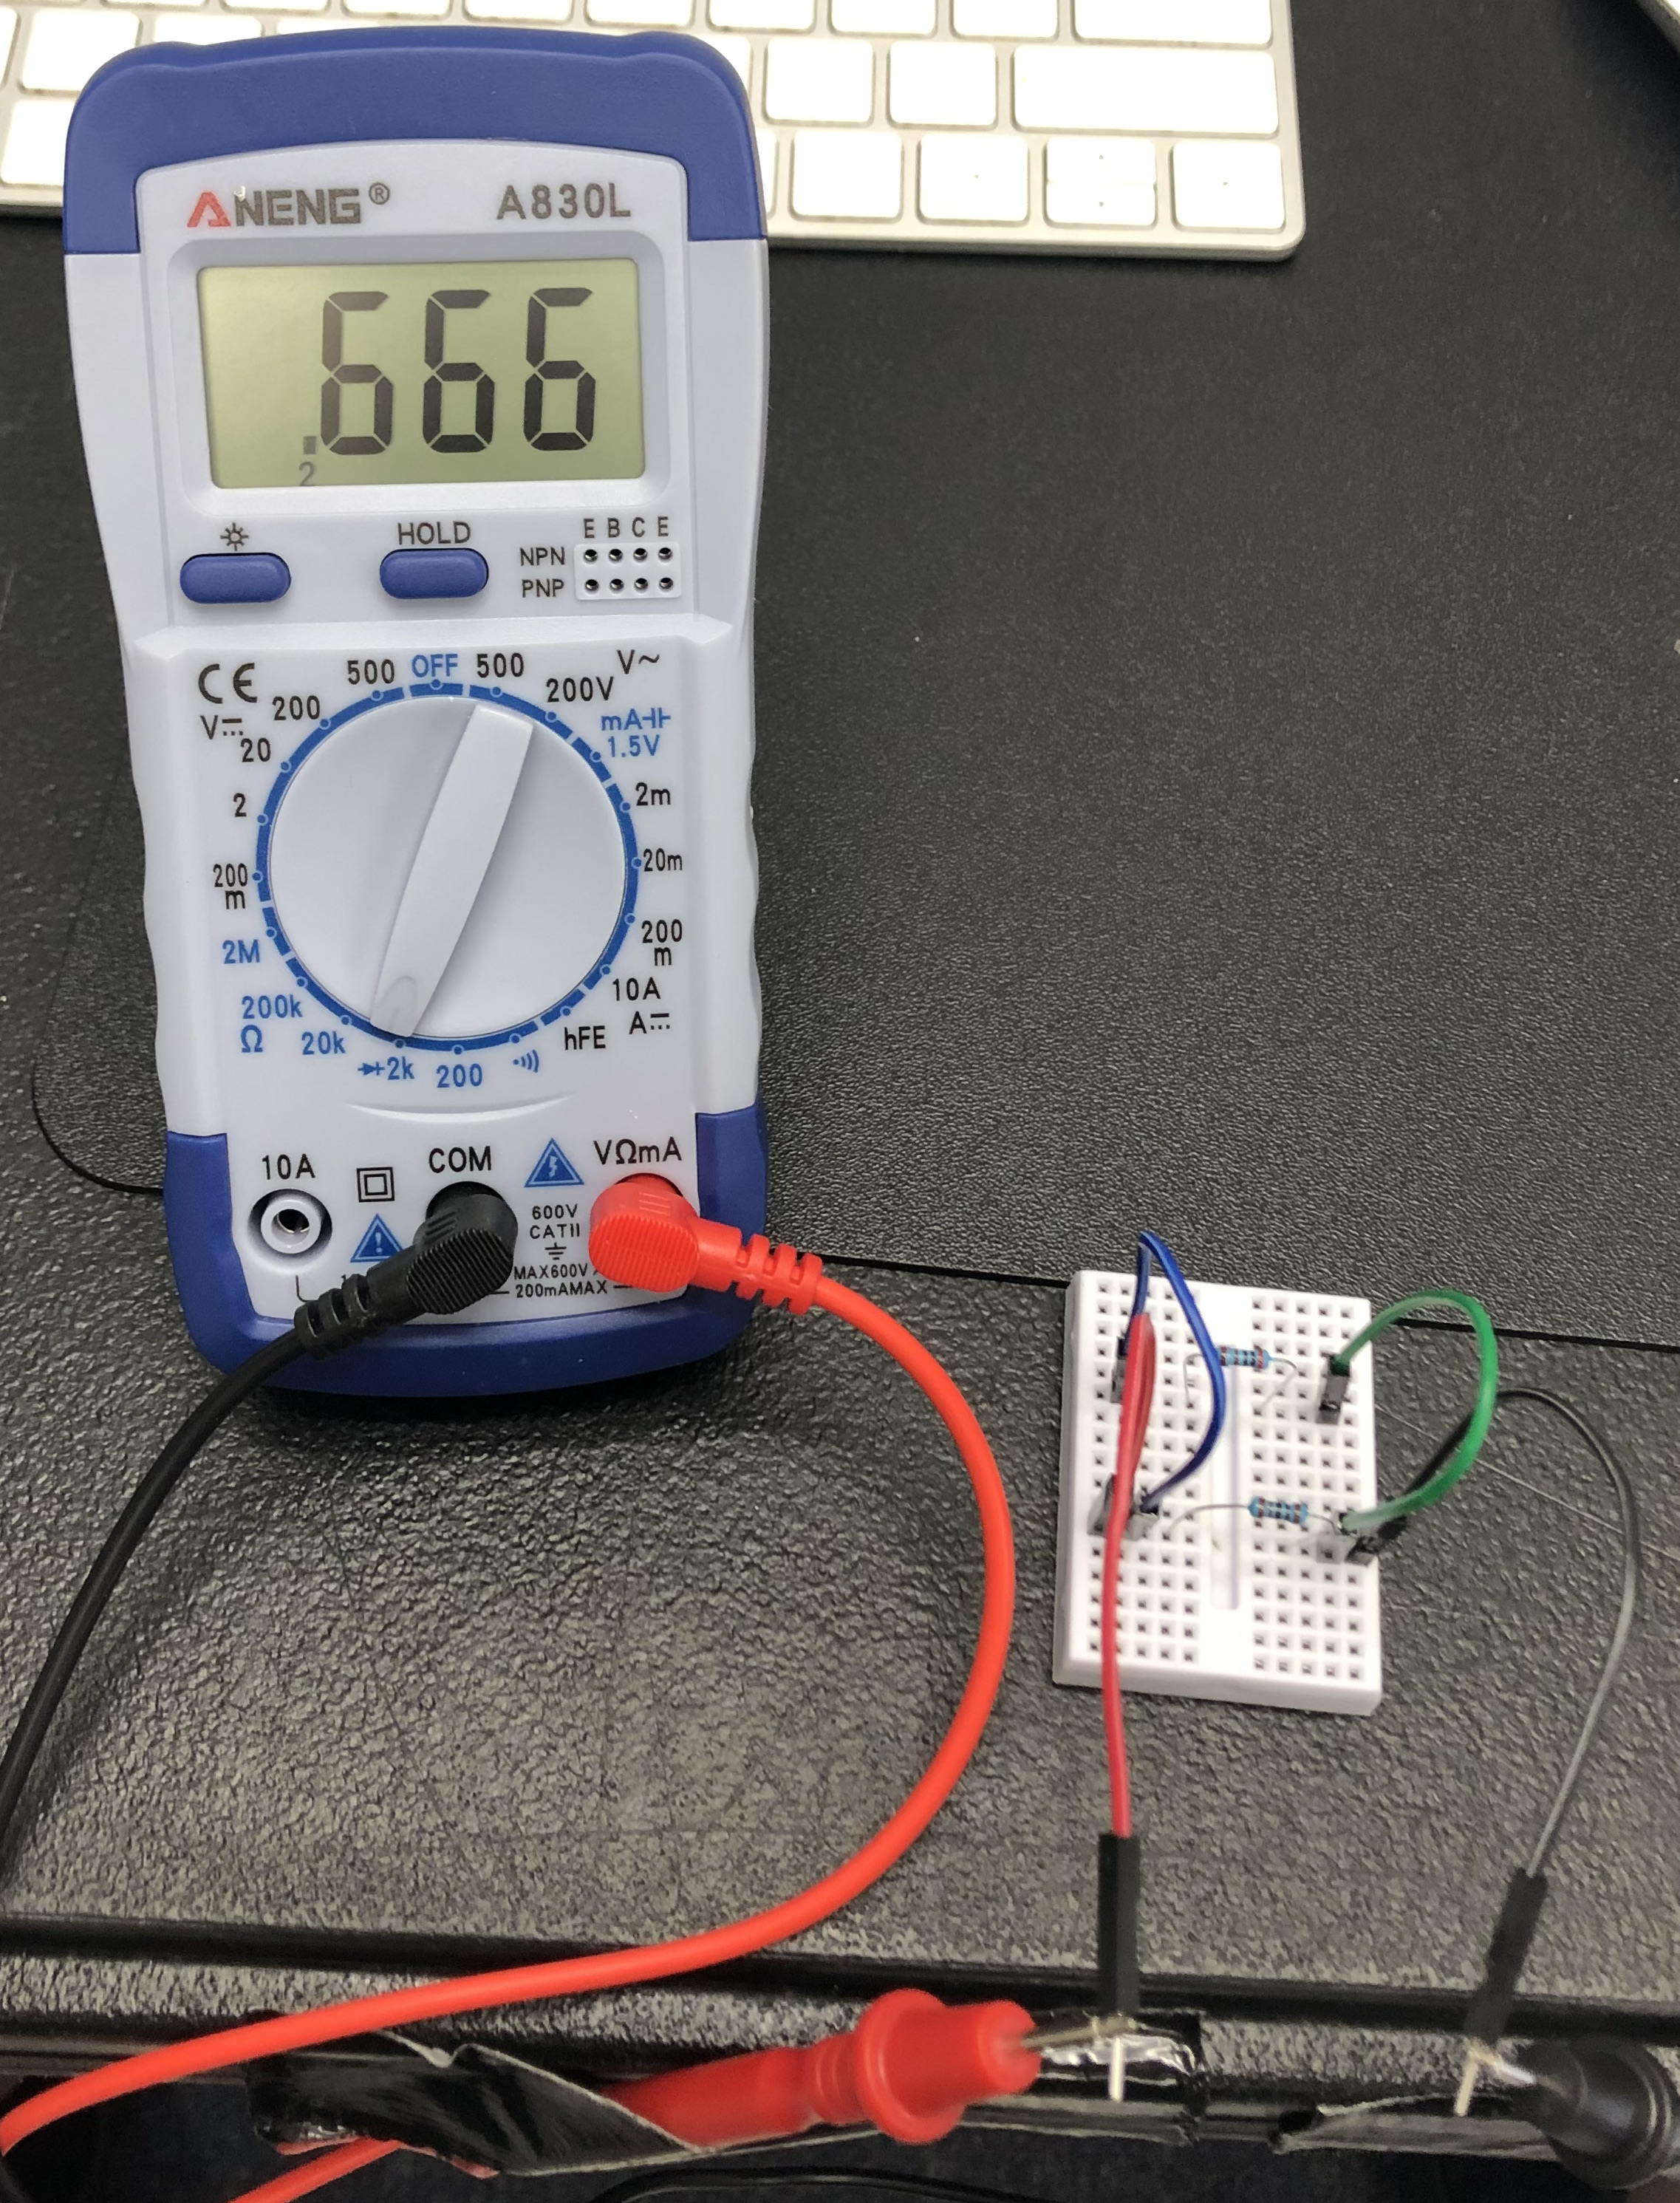
\includegraphics[scale=0.083,height=4.5cm]{RP.jpeg}
    \subsection*{Graph 1}
    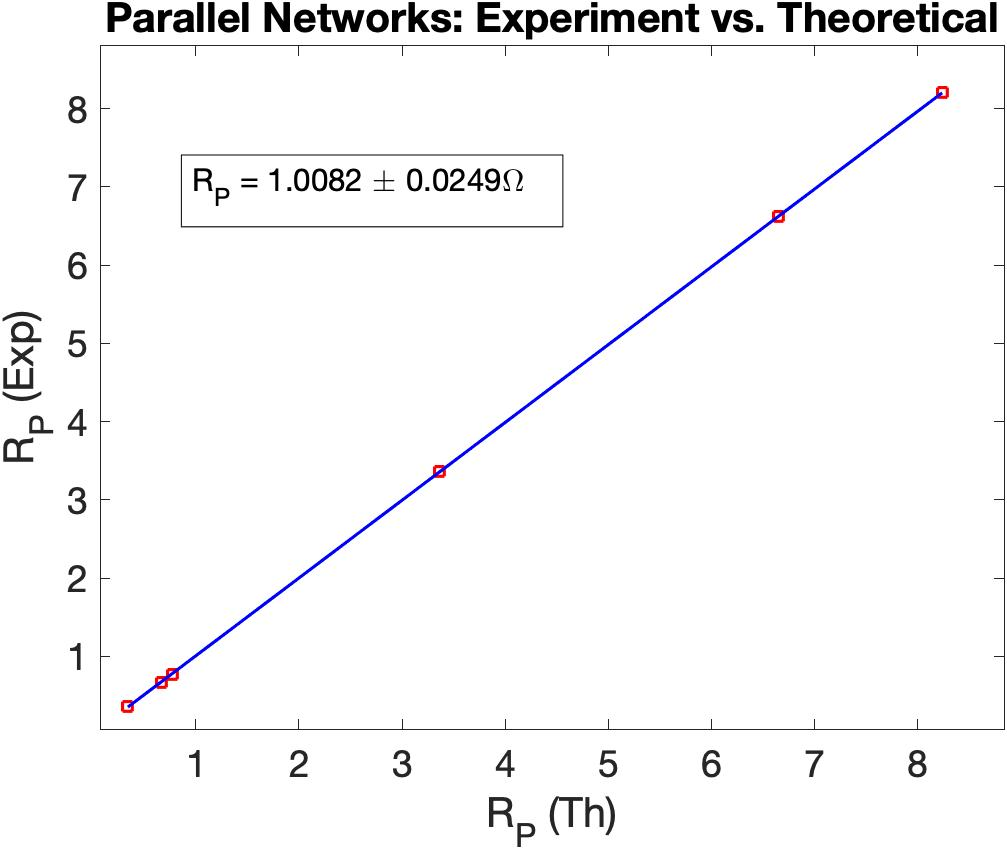
\includegraphics[scale=0.18]{parallel.jpeg}
    \subsection*{Discussion 1}
    \begin{enumerate}
      \item Discuss how well the experimental values of the parallel networks followed the theoretically expected value and quantify that relation.
      \begin{itemize}
        \item The experimental and theoretical values are relatively the same with less than 5\% difference proving that the voltages are same with currents \(i_1\) and \(i_2\) flowing through the split.
      \end{itemize}
    \end{enumerate}
  \end{center}
\end{table}
\newpage
\begin{table}[!htp]\centering
  \subsection*{Part 2}
  \begin{tabular}{|c|c|c|c|c|c|c|}\hline
  \multicolumn{6}{|c|}{\textbf{Table 2: Series Networks}} \\\hline
  \R{1}{th} & \R{1}{exp} & \R{2}{th} & \R{2}{exp} & \R{S}{th} & \R{S}{exp} \\\hline
  1k & 0.99k & 2k & 1.99k & 2.99k & 3.01k \\\hline
  1k & 0.99k & 510 & 0.51k & 1.51k & 1.52k \\\hline
  1k & 0.99k & 3.3k & 3.29k & 4.29k & 4.31k \\\hline
  10k & 9.97k & 5.1k & 5.07k & 15.04k & 14.98k \\\hline
  10k & 9.97k & 20k & 19.94k & 29.91k & 29.80k\\\hline
  10k & 9.97k & 47k & 47.40k & 57.37k & 57.40k \\\hline
  \end{tabular}
  \begin{center}
    \subsection*{Picture 2: \R{1}{exp},~\R{2}{exp},~\R{S}{exp}}
    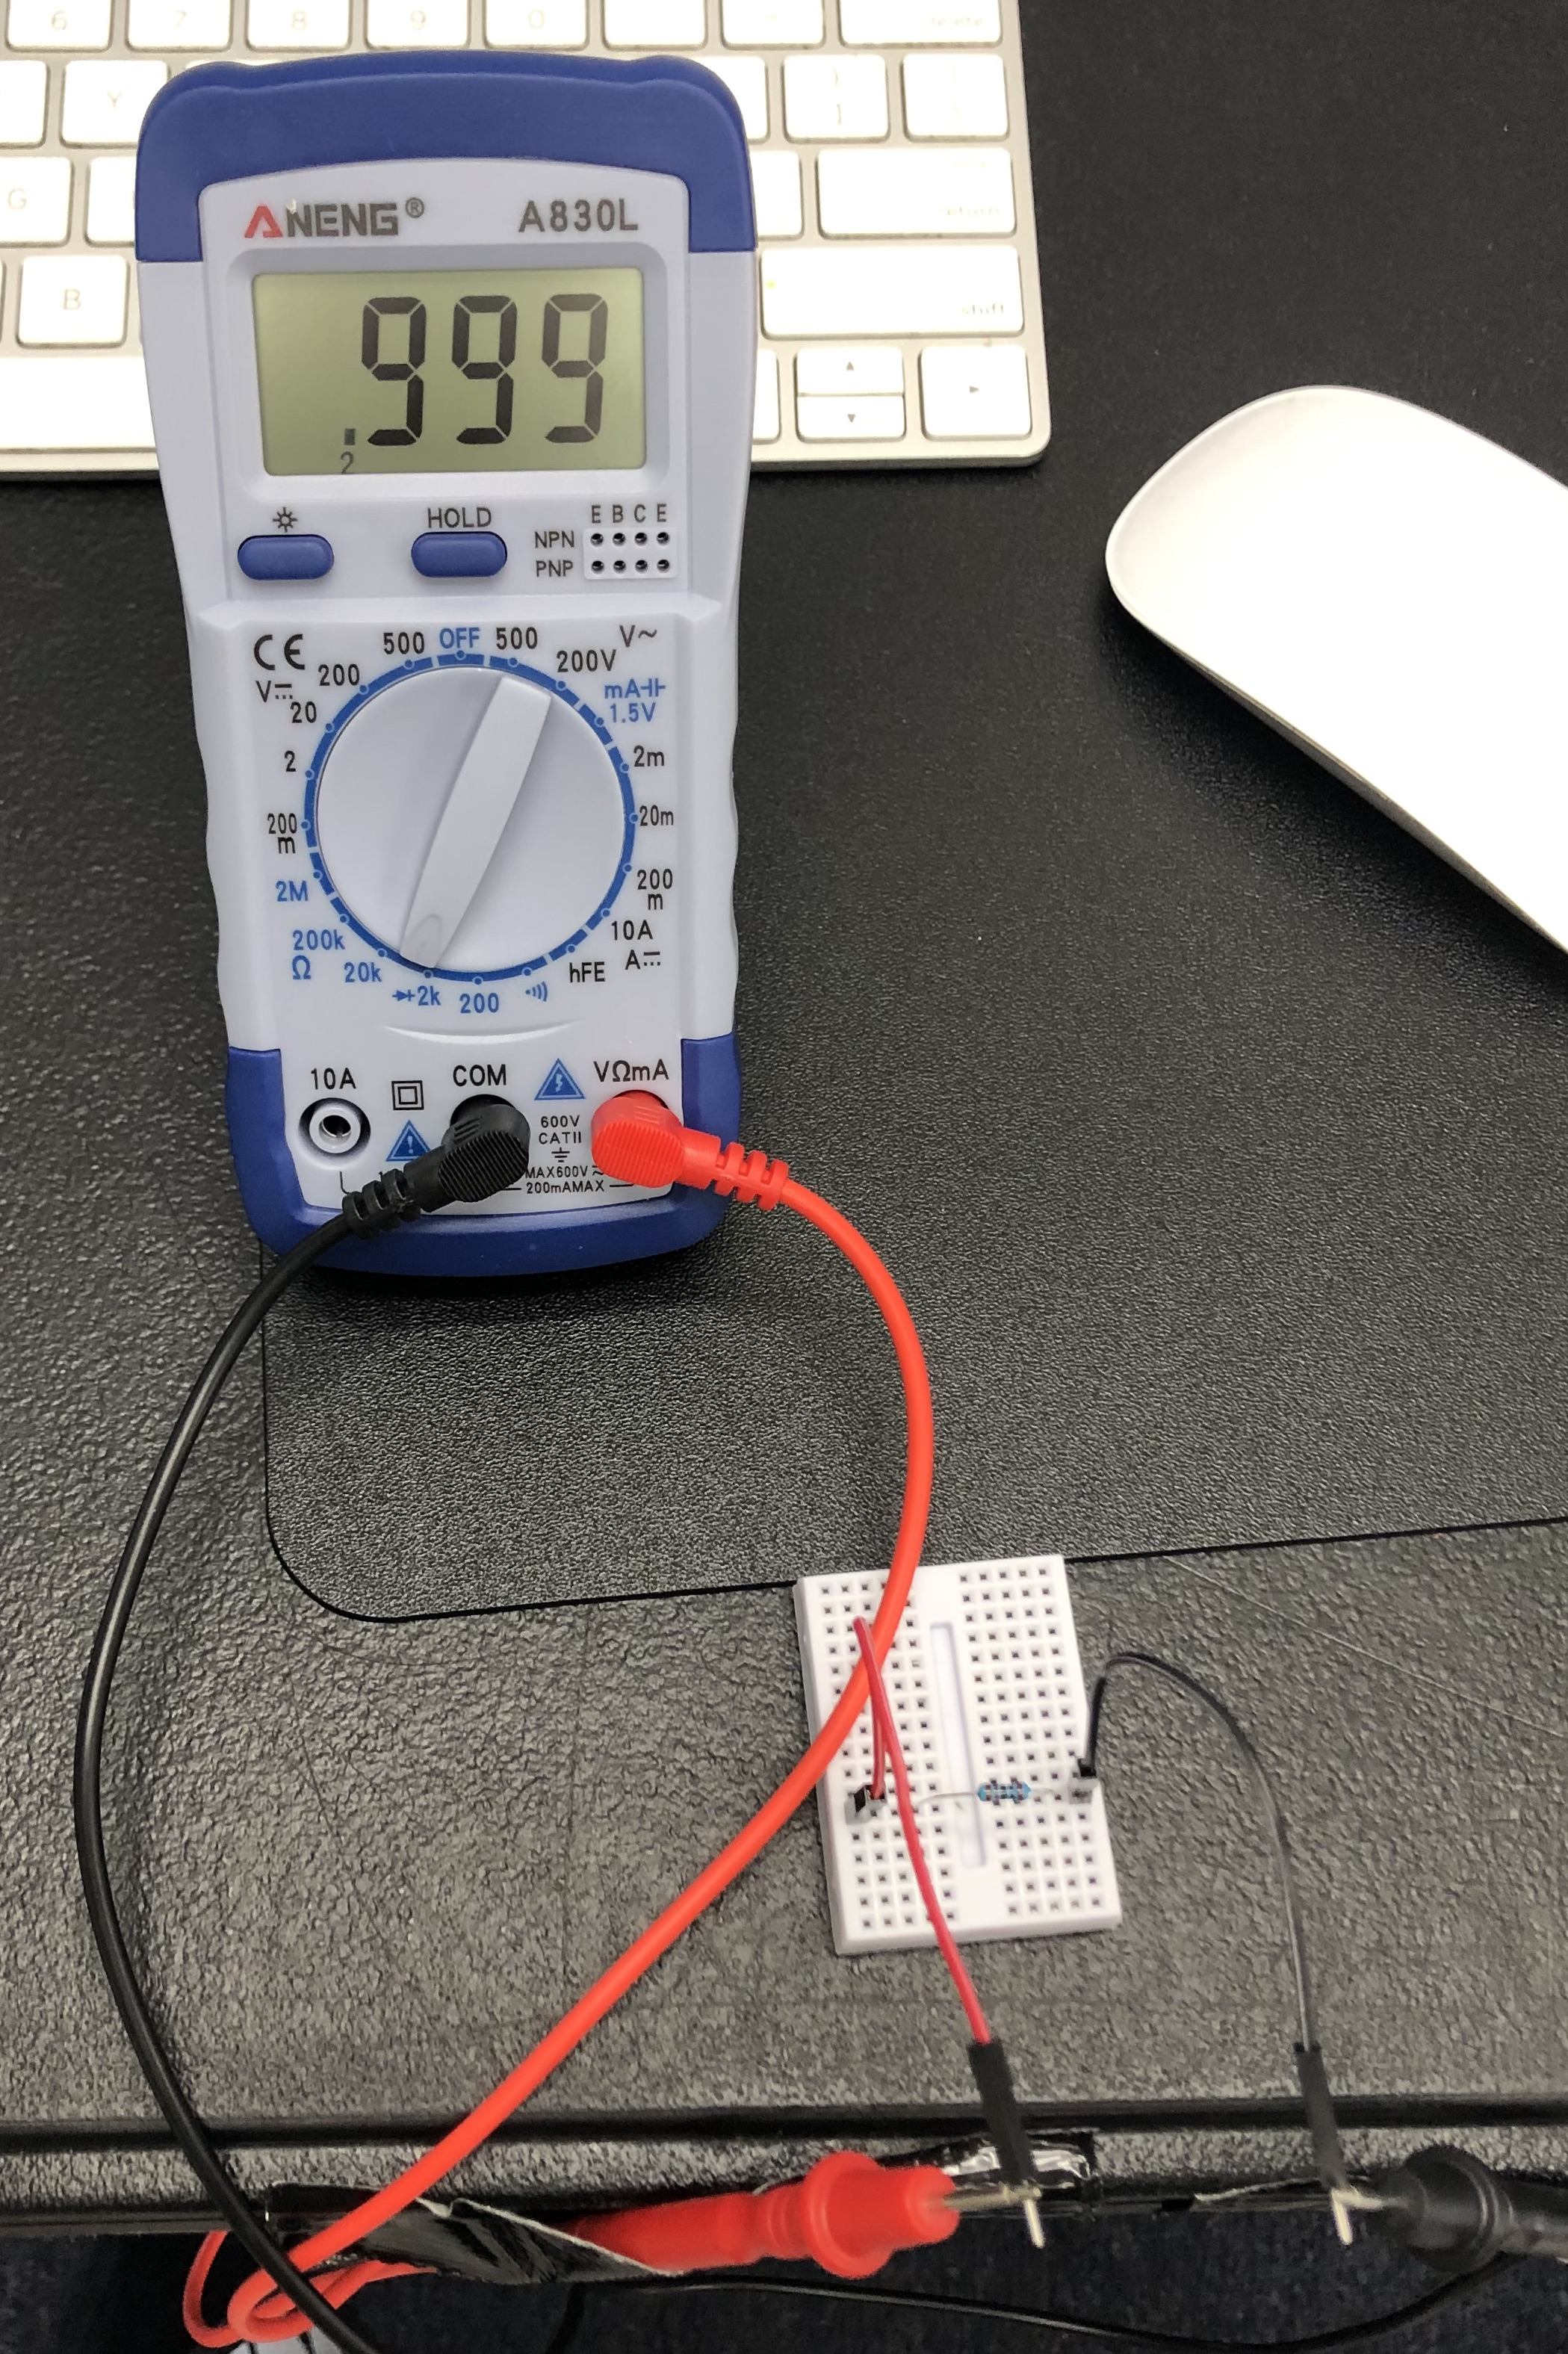
\includegraphics[scale=0.079,height=4.5cm]{R1.jpeg}
    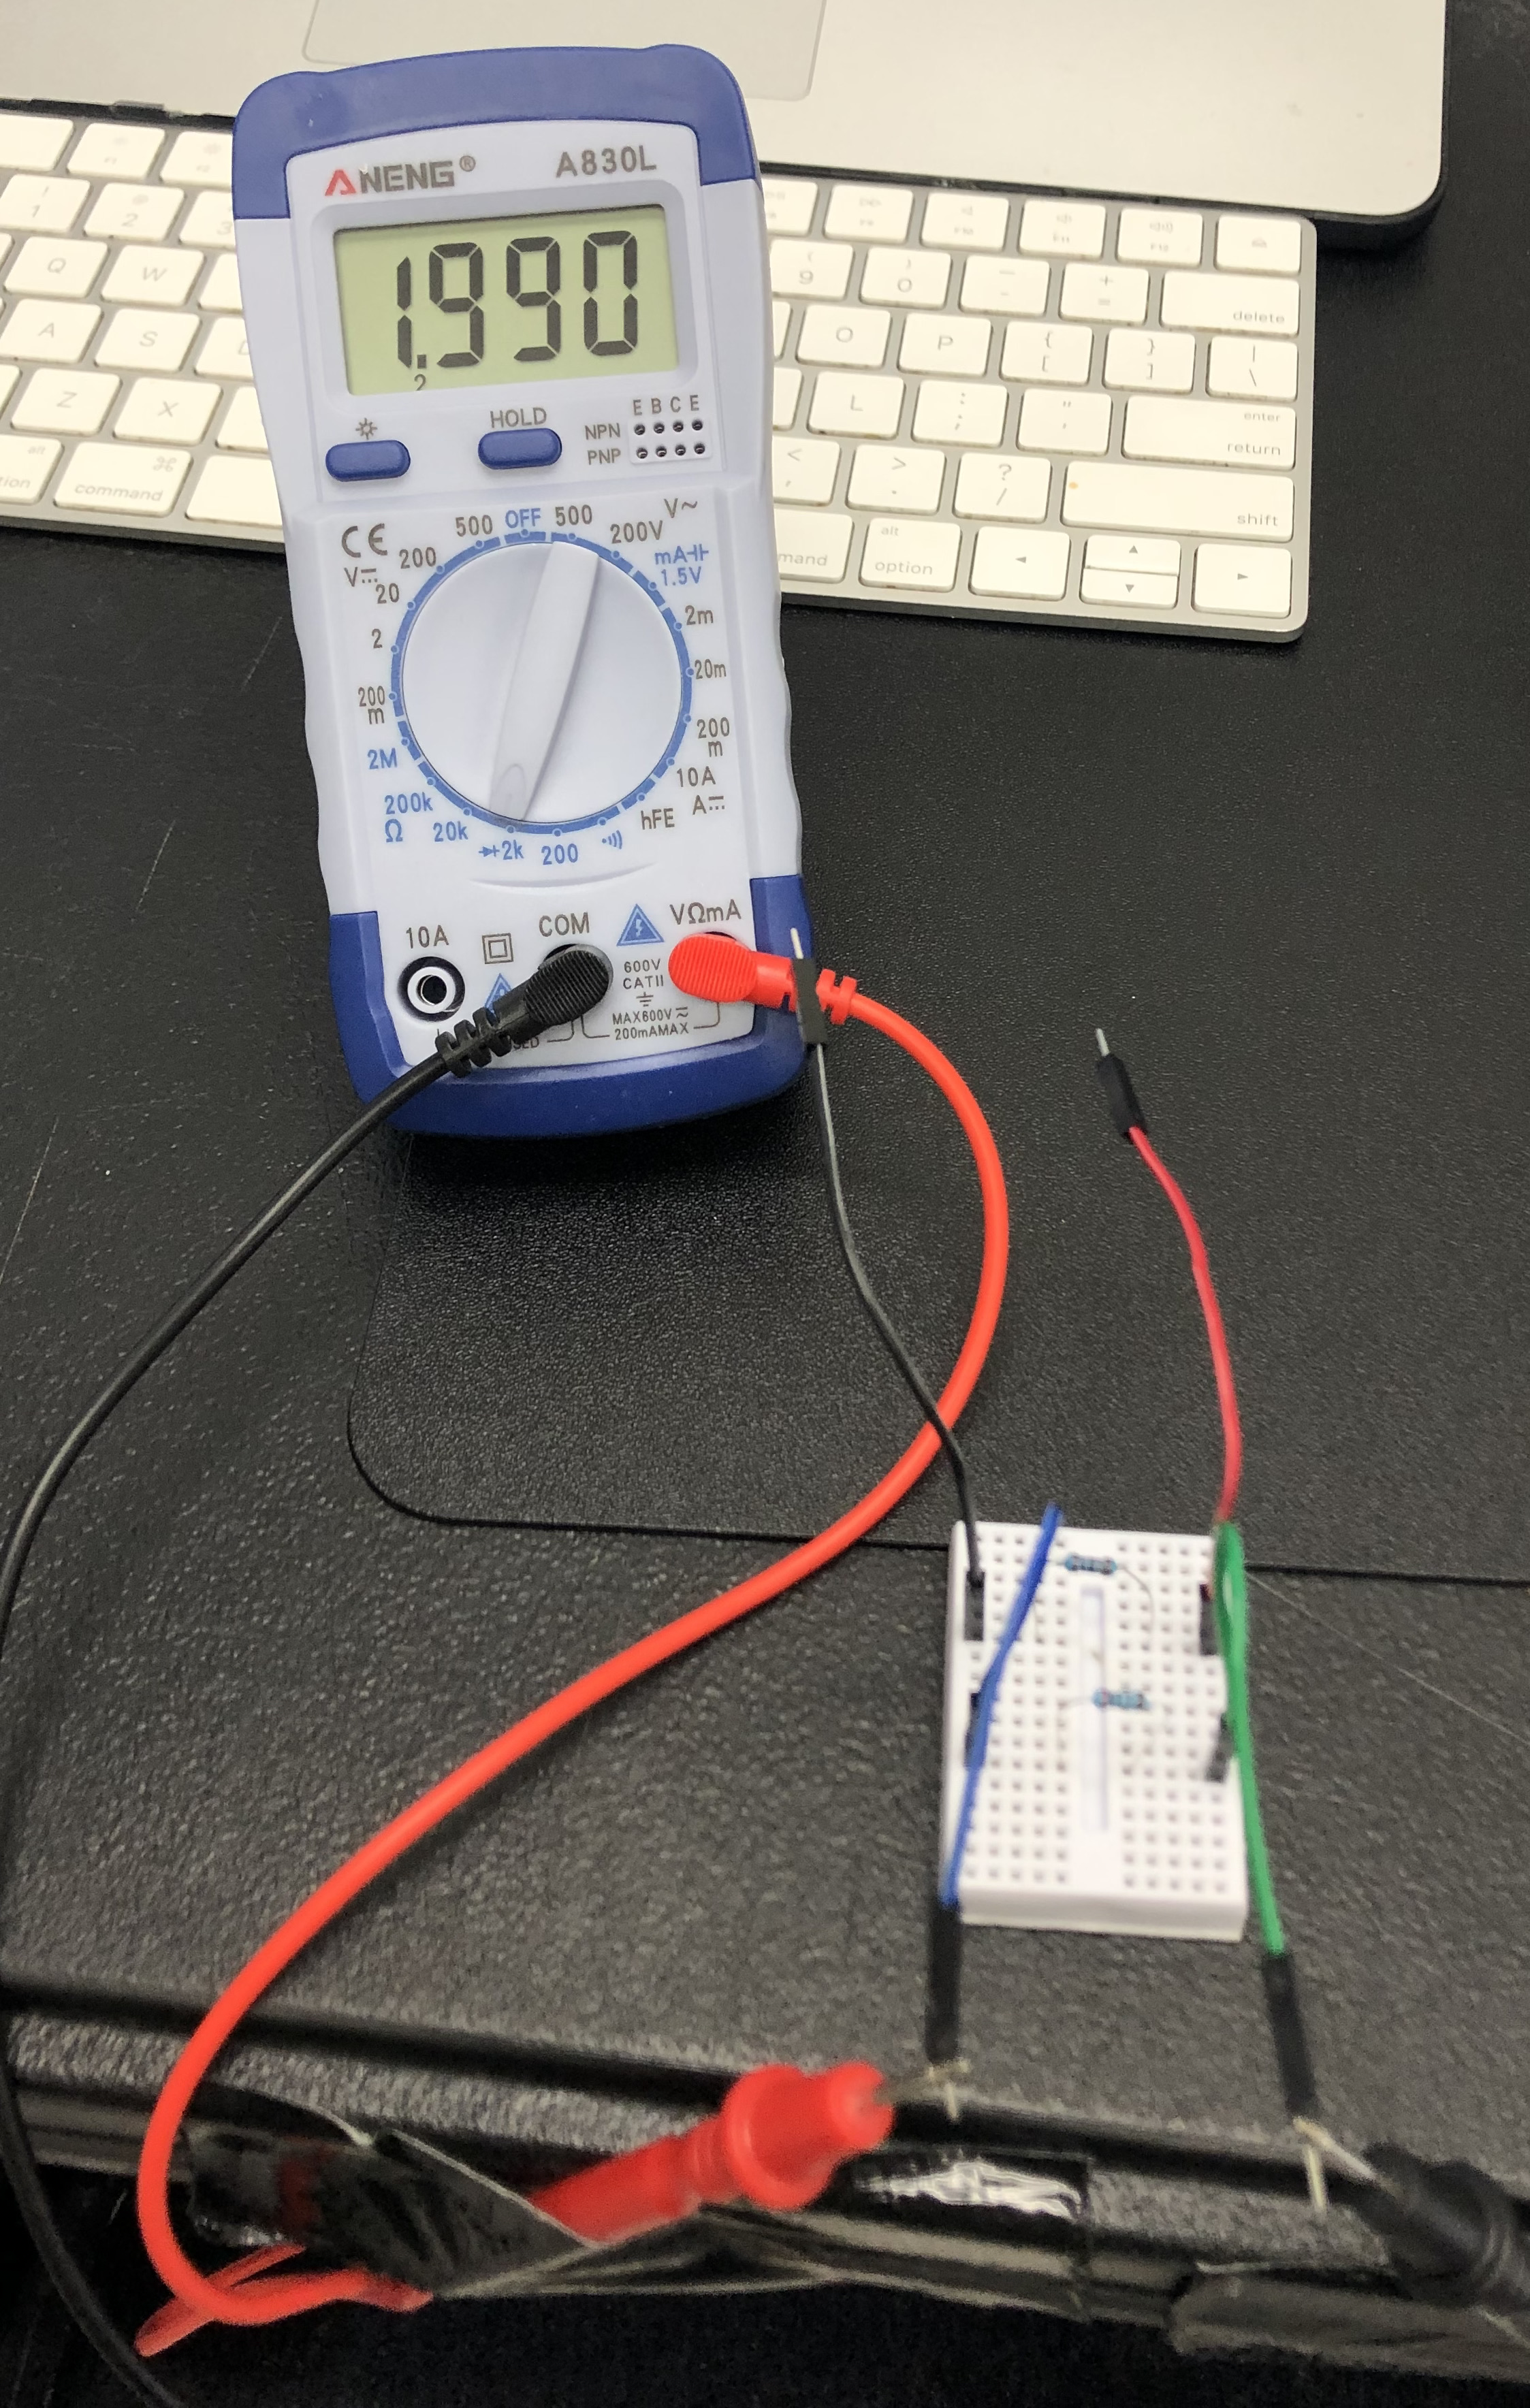
\includegraphics[scale=0.070,height=4.5cm]{R2.jpeg}
    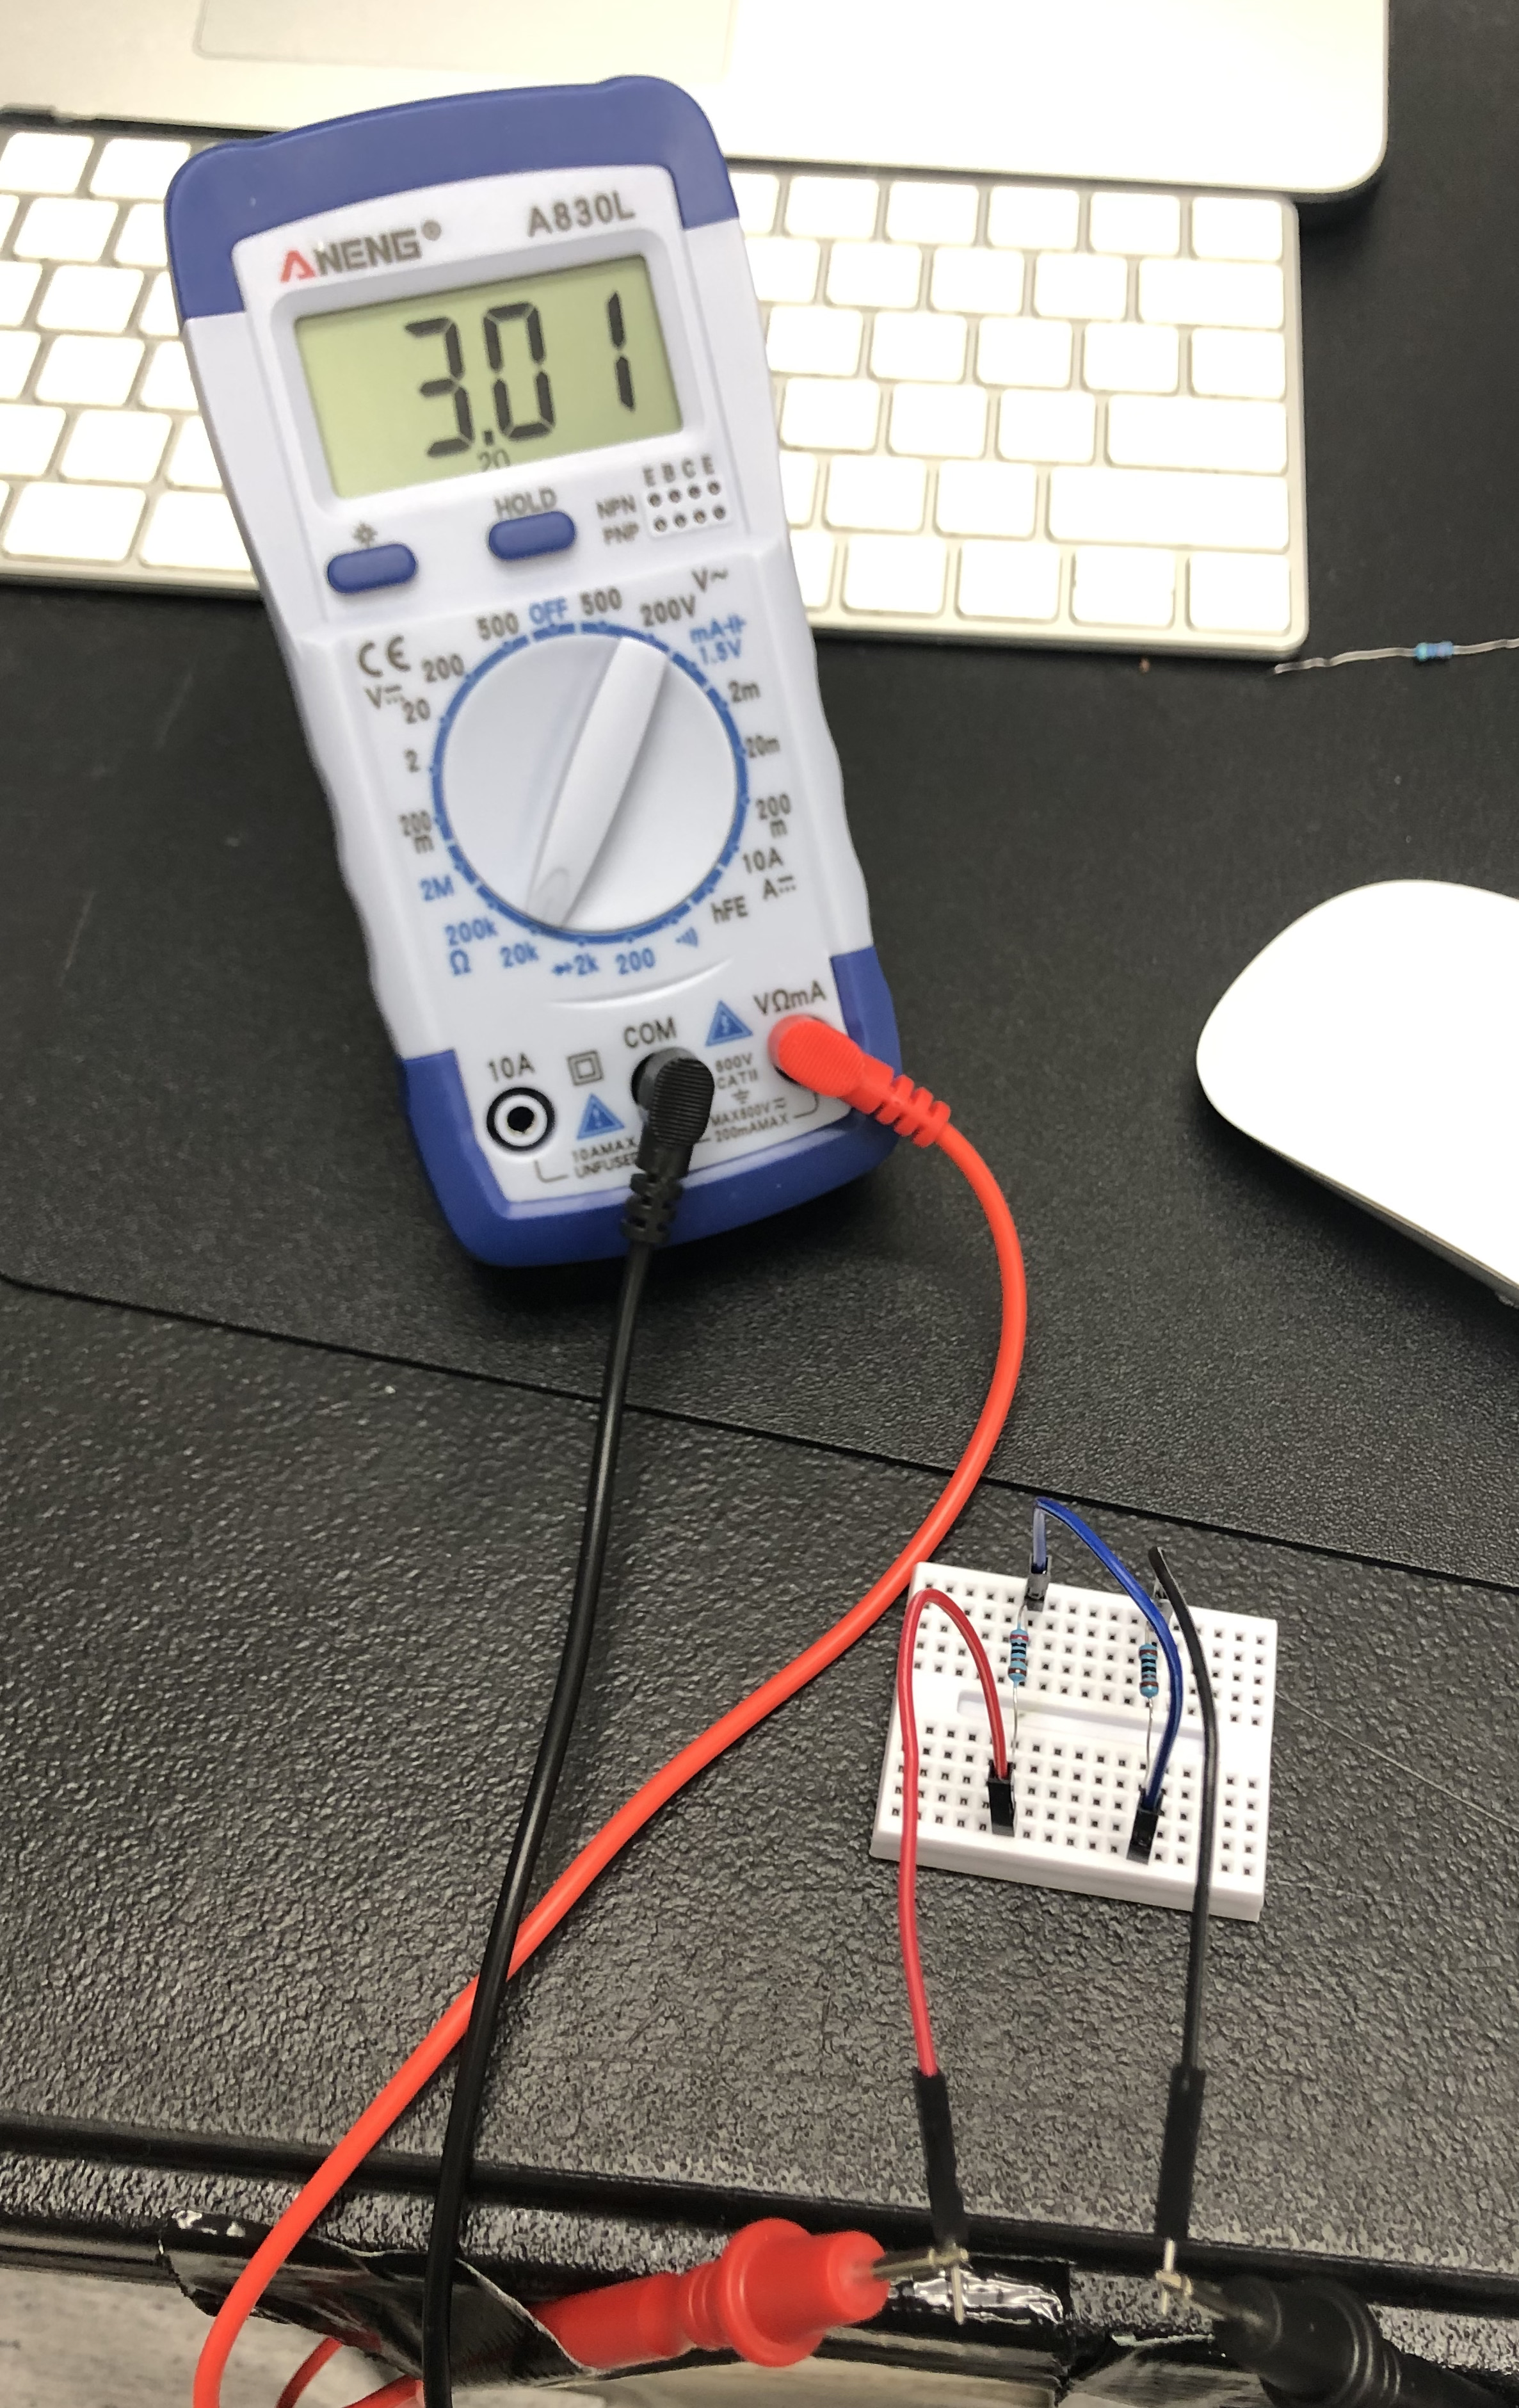
\includegraphics[scale=0.083,height=4.5cm]{RS.jpeg}
    \subsection*{Graph 2}
    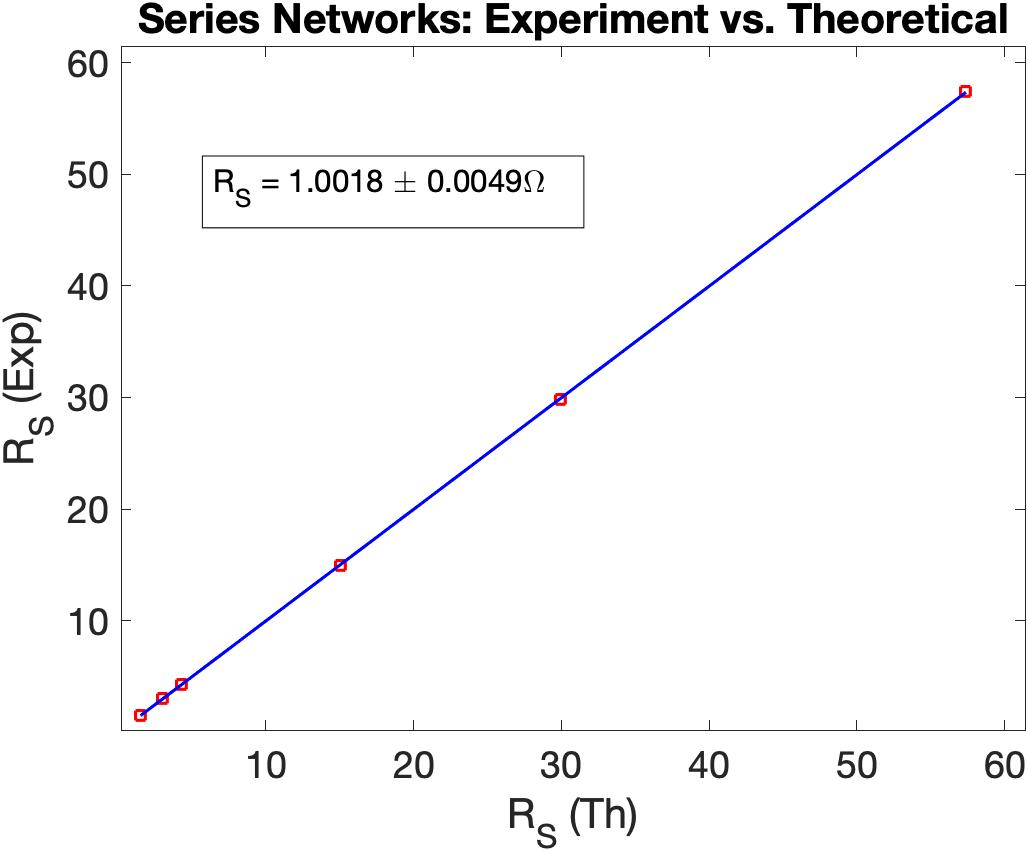
\includegraphics[scale=0.18]{series.jpeg}
    \subsection*{Discussion 2}
    \begin{enumerate}
      \item Discuss how well the experimental values of the series networks followed the theoretically expected value and quantify that relation.
      \begin{itemize}
        \item The experimental and theoretical values are relatively the same with less than 5\% difference proving that all charges that flow through \(R_1\) must also flow through \(R_2\), so currents \(i_1\) and \(i_2\) flowing through both is the same.
      \end{itemize}
    \end{enumerate}
  \end{center}
\end{table}
\end{document}